\section{Overview}\label{sec:overview}

This section provides a high-level overview of \tool. We describe the framework architecture (\autoref{sec:framework-overview}), walk through a motivating example (\autoref{sec:motivating-example}), and state the problem formally (\autoref{sec:problem-statement}).

\begin{figure}
    \centering
    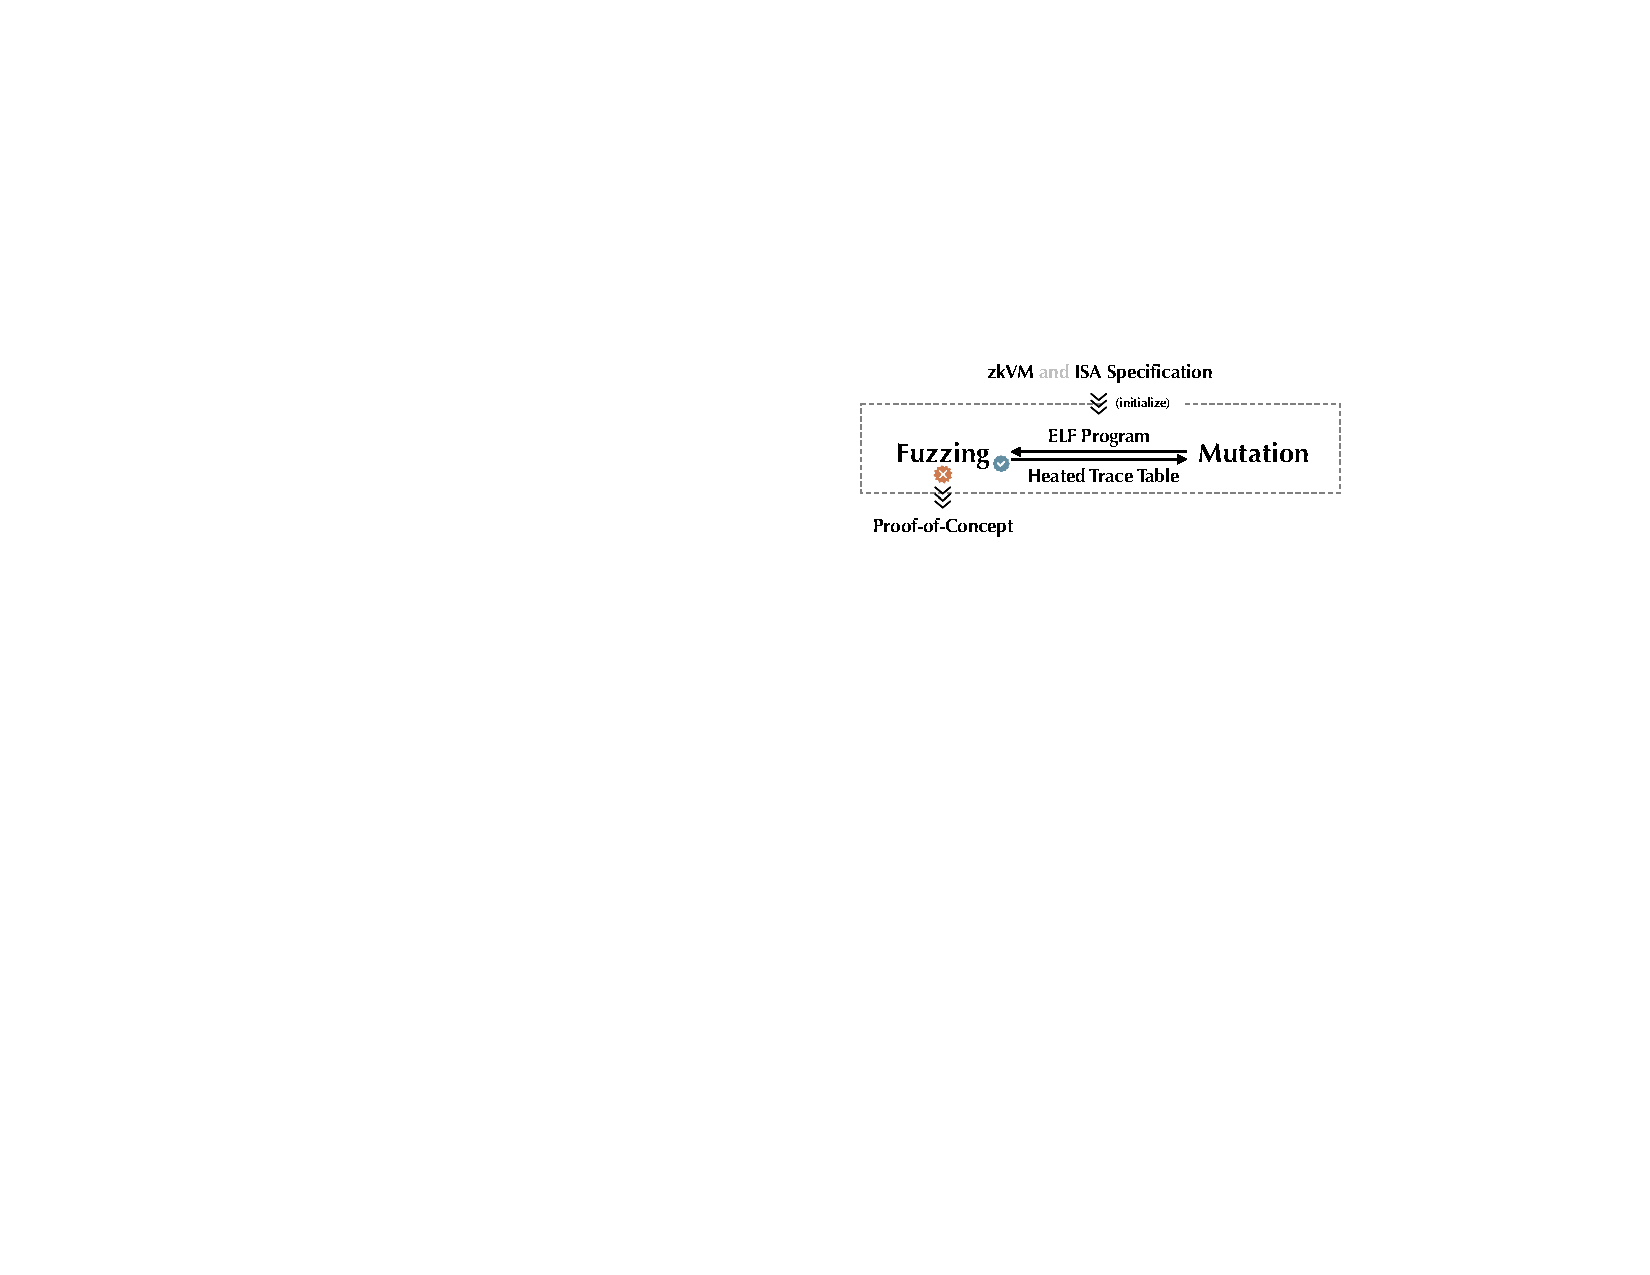
\includegraphics[width=\linewidth]{figs/overview.pdf}
    \caption{Architecture of \tool. Phase~1 performs signature-guided mutational fuzzing: RISC-V instruction sequences are mutated by an ISA-aware bandit, executed on both a reference oracle and the target zkVM backend, and projected through the semantic model to produce category signatures that guide further mutation. Phase~2 applies witness injection at constraint steps identified by the semantic model, detecting underconstrained circuits. Dashed arrows indicate feedback signals.}
    \label{fig:overview}
\end{figure}

\subsection{Framework Overview}\label{sec:framework-overview}

\autoref{fig:overview} illustrates the end-to-end architecture of \tool, which comprises two components. A \emph{cross-zkVM semantic model} (\autoref{sec:trace-ir}) lifts each backend's heterogeneous trace representation into a common vocabulary of constraint-correctness concerns, and a \emph{boundary-driven fuzzing framework} (\autoref{sec:fuzzing-framework}) uses that vocabulary to steer input generation toward underexplored boundary conditions.

The data flow proceeds as follows. A RISC-V instruction sequence is executed on both a reference oracle and the target zkVM backend. The backend's trace is projected through the semantic model to produce a \emph{category signature}: the set of constraint-correctness concerns activated by that execution. In \emph{Phase~1}, signature novelty replaces edge coverage as the fuzzing feedback signal, driving a UCB1 bandit that selects among eight ISA-aware mutation strategies. In \emph{Phase~2}, \tool probes each activated concern via targeted \emph{witness injection}, modifying the backend's internal witness to test whether the constraint system is underconstrained. The following example illustrates both phases on a real bug.

\subsection{Motivating Example}\label{sec:motivating-example}

We illustrate \tool's approach with a real constraint bug discovered in OpenVM's ALU chip: an \emph{immediate limb consistency} violation that allows a prover to decompose an immediate value into arbitrary limbs without constraint enforcement.

\paragraph{Background: immediate limb decomposition}
In OpenVM, the ALU chip processes each RISC-V instruction's immediate value by decomposing it into multiple limbs, i.e., small field elements whose product with appropriate powers of a base reconstructs the original value. For a 12-bit signed immediate (as in I-type instructions like \icode{addi}), the decomposition splits the value into byte-sized limbs. The circuit enforces a \emph{recomposition constraint}:
\begin{equation}\label{eq:recomp}
\mathit{limb}_0 + \mathit{limb}_1 \cdot 256 = \mathit{immediate}
\end{equation}
For instance, the immediate $-1$ (encoded as \icode{0xFFF} in the 12-bit two's complement) decomposes as $(\mathit{limb}_0, \mathit{limb}_1) = (\texttt{0xFF}, \texttt{0x0F})$, satisfying \autoref{eq:recomp}. To ensure a \emph{unique} decomposition, each limb must additionally be constrained to $[0, 255]$ via a range-check constraint:
\begin{equation}\label{eq:range}
0 \leq \mathit{limb}_i < 256 \quad \text{for each limb } i
\end{equation}

\paragraph{The bug}
Consider the instruction \icode{addi x1, x0, -1}, which sets register \icode{x1} to $-1$ (i.e., \icode{0xFFFF\_FFFF} in unsigned 32-bit representation). OpenVM's ALU chip enforced the recomposition constraint (\autoref{eq:recomp}) but \emph{omitted} the range-check constraint (\autoref{eq:range}) on the upper limb. This means the alternative decomposition $(\texttt{0xFF}, \texttt{0x1F})$ also satisfies the recomposition: $\texttt{0xFF} + \texttt{0x1F} \cdot 256 = \texttt{0x1FFF} \neq \texttt{0xFFF}$. Because the circuit uses the recomposed immediate to compute the instruction result, a malicious prover could claim that \icode{addi x1, x0, -1} stored a value derived from \icode{0x1FFF} rather than \icode{0xFFF}, forging a proof for an execution that never happened. The fix adds \icode{range\_check(limb\_i, 8)} for all limbs in the decomposition.

\paragraph{How \tool discovers this bug}
\tool's constant mutation arm (Arm~2) replaces an immediate with $-1$, a boundary value it prioritizes. The instrumented backend emits an \icode{ImmediateLimbObservation}, classified under \icode{alu.imm\_limb}. If this produces a novel category signature, the input enters the corpus. In Phase~2, \tool arms an injection replacing the limb values with an alternative decomposition and observes that the circuit accepts---confirming an \emph{underconstrained candidate}. The reference oracle simultaneously reports the correct value (\icode{0xFFFF\_FFFF}); the mismatch under the injected witness is recorded as a bug.

\paragraph{Why existing approaches miss this bug}
Generic fuzzing (\arguzz) is unlikely to generate immediate $-1$ \emph{and} exercise the specific ALU path; static analysis (\zkap) lacks trace-table structure to reason about limb consistency. \tool succeeds because (1)~ISA-aware mutation targets boundary immediates, (2)~the semantic model names this condition via \icode{alu.imm\_limb}, and (3)~witness injection validates constraint soundness directly.

\subsection{Problem Statement}\label{sec:problem-statement}

We now state the problem that \tool addresses.

\paragraph{Setting}
Let $O$ denote a reference RISC-V oracle that faithfully implements the RV32IM instruction set, and let $B$ denote a zkVM backend with arithmetization $A$. Given a RISC-V instruction sequence $x = (\iota_1, \ldots, \iota_n)$ where each $\iota_i$ is a 32-bit instruction word, $O(x)$ and $B(x)$ each produce a final register state $r \in \mathbb{Z}_{2^{32}}^{32}$ (a vector of 32 unsigned 32-bit integers).

\paragraph{Goal}
Find inputs $x$ such that either:
\begin{enumerate}
    \item \textbf{Semantic divergence:} $O(x) \neq B(x)$, indicating that the backend's execution trace corresponds to a different computation than the RISC-V specification prescribes; or
    \item \textbf{Underconstrained circuit:} there exists a witness injection $I_{b,s}$ (for some category $b$ and step $s$) such that $B$ accepts the altered witness without error, indicating that the arithmetization $A$ is insufficiently constrained at the boundary condition identified by category $b$.
\end{enumerate}

\paragraph{Challenges}
The search space is exponentially large, divergences occur at rare boundary conditions unreachable by random testing, and heterogeneous trace representations preclude a single testing methodology (\autoref{sec:bg-challenges}). \tool addresses these via the semantic model (unifying traces) and boundary-driven fuzzing (steering exploration).
